\subsection{Summary}

\subsection{Recommended Use Cases}
One of the most known users of a \chuk derivate is \textbf{Netflix}. 

\label{netflix}
\begin{figure}[hbt]
  \centering
  % https://drive.google.com/open?id=1Nmn-mWvxAwhcB9Vo4nbq0gutnWp0bPcCfBU14KMDVQ8
  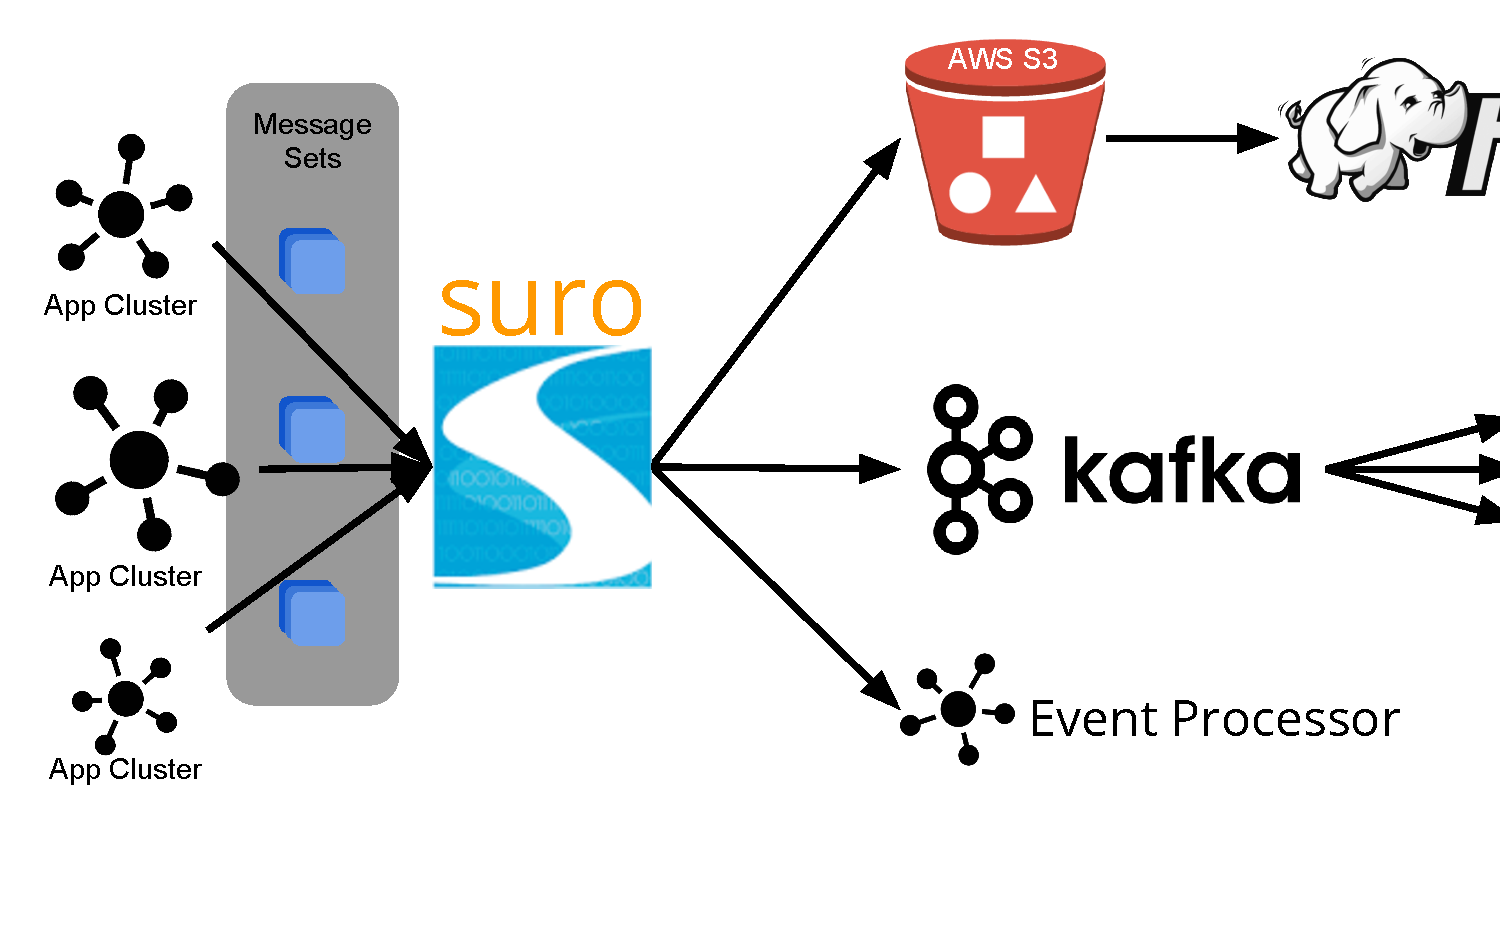
\includegraphics[width=\linewidth,clip=true,trim=5mm 2cm 0 5mm]{images/NetflixSuro}
  \caption{Netflix Suro Architecture~\cite{Bae2013, Harris2013}}
  \label{fig:SuroArchitecture}
\end{figure}


\subsection{Feature Research Questions}
Current research has not shown, in which extend the two systems \amblong and \chuk can be used in an inter-connected manner, complementing each others services. Managing large, internet-scale clusters, consisting of multiple thousand hosts running \hadooplong can be more automated and controlled with Systems like \amb and \chuk in place, not only controlling the current state, but also managing installed components and archiving system-state information.

Further, an improved way of storing Chukwas log data in a more structured way, allowing live querying, is still be to found. Boulon et al. did look into several options so far~\cite{Boulonb}, but this work has to be continued.

Last, but not least, the real-time approach shown in \ref{netflix} may be extended, as the ``recent trend has been in the area of real-time stream processing''~\cite{Bae2013} and will most likely continue in the future.